%Edit 0040 ZZZ to report number nnnn 
%Edit 5.1 YYMILE to milestone number m.m.m
%Edit Management of external research. Supports UQ Procurement YYTITLE to report title - Words Start with Caps
\documentclass[11pt,twoside,a4paper]{article}
%%======================================================================
%% PACKAGES:
%%
%\usepackage{times}               % Times+Helvetica+Courier fonts
\usepackage{helvet}              % helvetica + cmr
\usepackage{fancyhdr}       % package for headers/footers
\usepackage{amsmath}
\usepackage{amssymb}
\usepackage{graphicx}            % Graphics.
%\usepackage{a4}                  % page layout to fit A4
%\usepackage{lastpage}            % get page no of last page
%\usepackage{ifthen}              % logical branching
\usepackage{hyperref}            %insert hyper-links
\usepackage{latexsym}
% uncomment the following to override auto page total
%\pptotal{20}
%%======================================================================

% Script lifted from Quora answer
% https://www.quora.com/What-is-the-optimal-way-to-include-Python-code-in-a-LaTeX-document

\usepackage{color} 
\usepackage{listings}
\usepackage{setspace}

 \definecolor{Code}{rgb}{0,0,0}
 \definecolor{Decorators}{rgb}{0.5,0.5,0.5}
 \definecolor{Numbers}{rgb}{0.5,0,0}
 \definecolor{MatchingBrackets}{rgb}{0.25,0.5,0.5}
 \definecolor{Keywords}{rgb}{0,0,1}
 \definecolor{self}{rgb}{0,0,0}
 \definecolor{Strings}{rgb}{0,0.63,0}
 \definecolor{Comments}{rgb}{0,0.63,1}
 \definecolor{Backquotes}{rgb}{0,0,0}
 \definecolor{Classname}{rgb}{0,0,0}
 \definecolor{FunctionName}{rgb}{0,0,0}
 \definecolor{Operators}{rgb}{0,0,0}
 \definecolor{Background}{rgb}{0.98,0.98,0.98}

  \lstdefinelanguage{Python}{
  numbers=left,
  numberstyle=\footnotesize,
  numbersep=1em,
  xleftmargin=1em,
  framextopmargin=2em,
  framexbottommargin=2em,
  showspaces=false,
  showtabs=false,
  showstringspaces=false,
  frame=l,
  tabsize=4,
  % Basic
  basicstyle=\ttfamily\small\setstretch{1},
  backgroundcolor=\color{Background},
  % Comments
  commentstyle=\color{Comments}\slshape,
  % Strings
  stringstyle=\color{Strings},
  morecomment=[s][\color{Strings}]{"""}{"""},
  morecomment=[s][\color{Strings}]{'''}{'''},
  % keywords
  morekeywords={import,from,class,def,for,while,if,is,in,elif,else,not,and,or,print,break,continue,return,True,False,None,access,as,,del,except,exec,finally,global,import,lambda,pass,print,raise,try,assert},
  keywordstyle={\color{Keywords}\bfseries},
  % additional keywords
  morekeywords={[2]@invariant,pylab,numpy,np,scipy},
  keywordstyle={[2]\color{Decorators}\slshape},
  emph={self},
  emphstyle={\color{self}\slshape},
  %
  }



% ensure sans-serif font used throughout
\renewcommand{\familydefault}{\sfdefault}

\newcommand{\culhamissueno}{1.00}%<==edit
\newcommand{\culhamshorttitle}{CD/EXCALIBUR-FMS/0040}%<==edit
\newcommand{\Sec}[1]{Section~\ref{sec:#1}}
\newcommand{\Fig}[1]{Figure~\ref{fig:#1}}
\newcommand{\Tab}[1]{Table~\ref{tab:#1}}
\newcommand{\Eq}[1]{Equation~(\ref{eq:#1})}
\newcommand{\Eqs}[2]{Equations(\ref{eq:#1}) and~(\ref{eq:#2})}
\newcommand{\Figs}[2]{Figures~\ref{fig:#1}--~\ref{fig:#2}}
%Bold lc for script names, tt for computer code and file-names
%\F{NEPTUNE} always in caps
\newcommand{\F}[1]{\textsc{#1}}
\newcommand{\B}[1]{\textbf{#1}}
\newcommand{\T}[1]{{\tt #1}}
\newcommand{\V}[1]{\mathbf{#1}}
\newcommand{\I}[1]{\textit{#1}}
\newcommand{\nep}{\textsc{NEPTUNE}}
\newcommand{\exc}{\textsc{E}x\textsc{CALIBUR}}
\newcommand{\Papp}{Proxyapp}
\newcommand{\papp}{proxyapp}



%%======================================================================

%% REPORT COVER PAGE Information

\newcommand{\culhamtitle}{\LARGE Management of external research. Supports UQ Procurement  \\[1.0\baselineskip] M5.1 }%<==edit

%%QA BOX information -- change following as needed
\newcommand{\culhamboardname}{Martin O'Brien}%<==edit
\newcommand{\culhamcontactname}{Rob Akers}%<==edit
\newcommand{\culhamauthor}{Wayne Arter}%<==edit
\newcommand{\culhamauthora}{Ed Threlfall}%<==edit
\newcommand{\culhamauthorb}{Joseph Parker}%<==edit
\newcommand{\culhamauthorc}{Will Saunders}%<==edit
%\newcommand{\culhamcontacttel}{Telephone: 01235 466498}
%\newcommand{\culhamcontactemail}{Email: rob.akers@ukaea.uk}

\newcommand{\culhamdate}{\today}%<=edit
\newcommand{\culhamdatea}{\today}%<=edit
\newcommand{\culhamdateb}{\today}%<=edit

% reproduce Rob's page size

\setlength{\textheight}{220.0mm}
\setlength{\textwidth}{165.0mm}
\setlength{\topmargin}{0.0mm}
\setlength{\oddsidemargin}{0.0mm}
\setlength{\evensidemargin}{\oddsidemargin}
\setlength{\parindent}{0mm}
\addtolength{\parskip}{0.5\baselineskip}
\setlength{\topsep}{0pt}
\setlength{\itemsep}{0pt}

%%======================================================================
\begin{document}

%Titlepage comes out wrong size, but should look right apart from
% picture which cannot be wider than c.150mm.
% To produce conforming report rp1pub.pdf
% remove title page by commenting out lines ending in %<==omit, then
% sed -e '/<==omit$/s/^/%/' < rp1.tex > rp1omit.tex
% pdflatex rp1omit;bibtex rp1omit; pdflatex rp1omit
% pdfunite cover.pdf rp1omit.pdf rp1pub.pdf 
\begin{titlepage}%<==omit
\vspace*{-30mm}%<==omit

\includegraphics[width=2.5cm]{../corpics/cofaplus} \\[2.0\baselineskip]%<==omit
{\LARGE {\textbf{\textsf{ExCALIBUR}}}}\\[2.0\baselineskip]%<==omit
{\LARGE \culhamtitle } \\[2.0\baselineskip]%<==omit
{\textbf{\textsf{Abstract}}}\\%<==omit
The report describes work for \exc \ project \nep \ %<==omit
at Milestone 5.1. %<==omit
Report on the status of programming models and code generators for the
various node architectures focused on performance, usability, maintainability
and  availability.  
%<==omit
%<==omit
\vfill%<==omit
\centerline{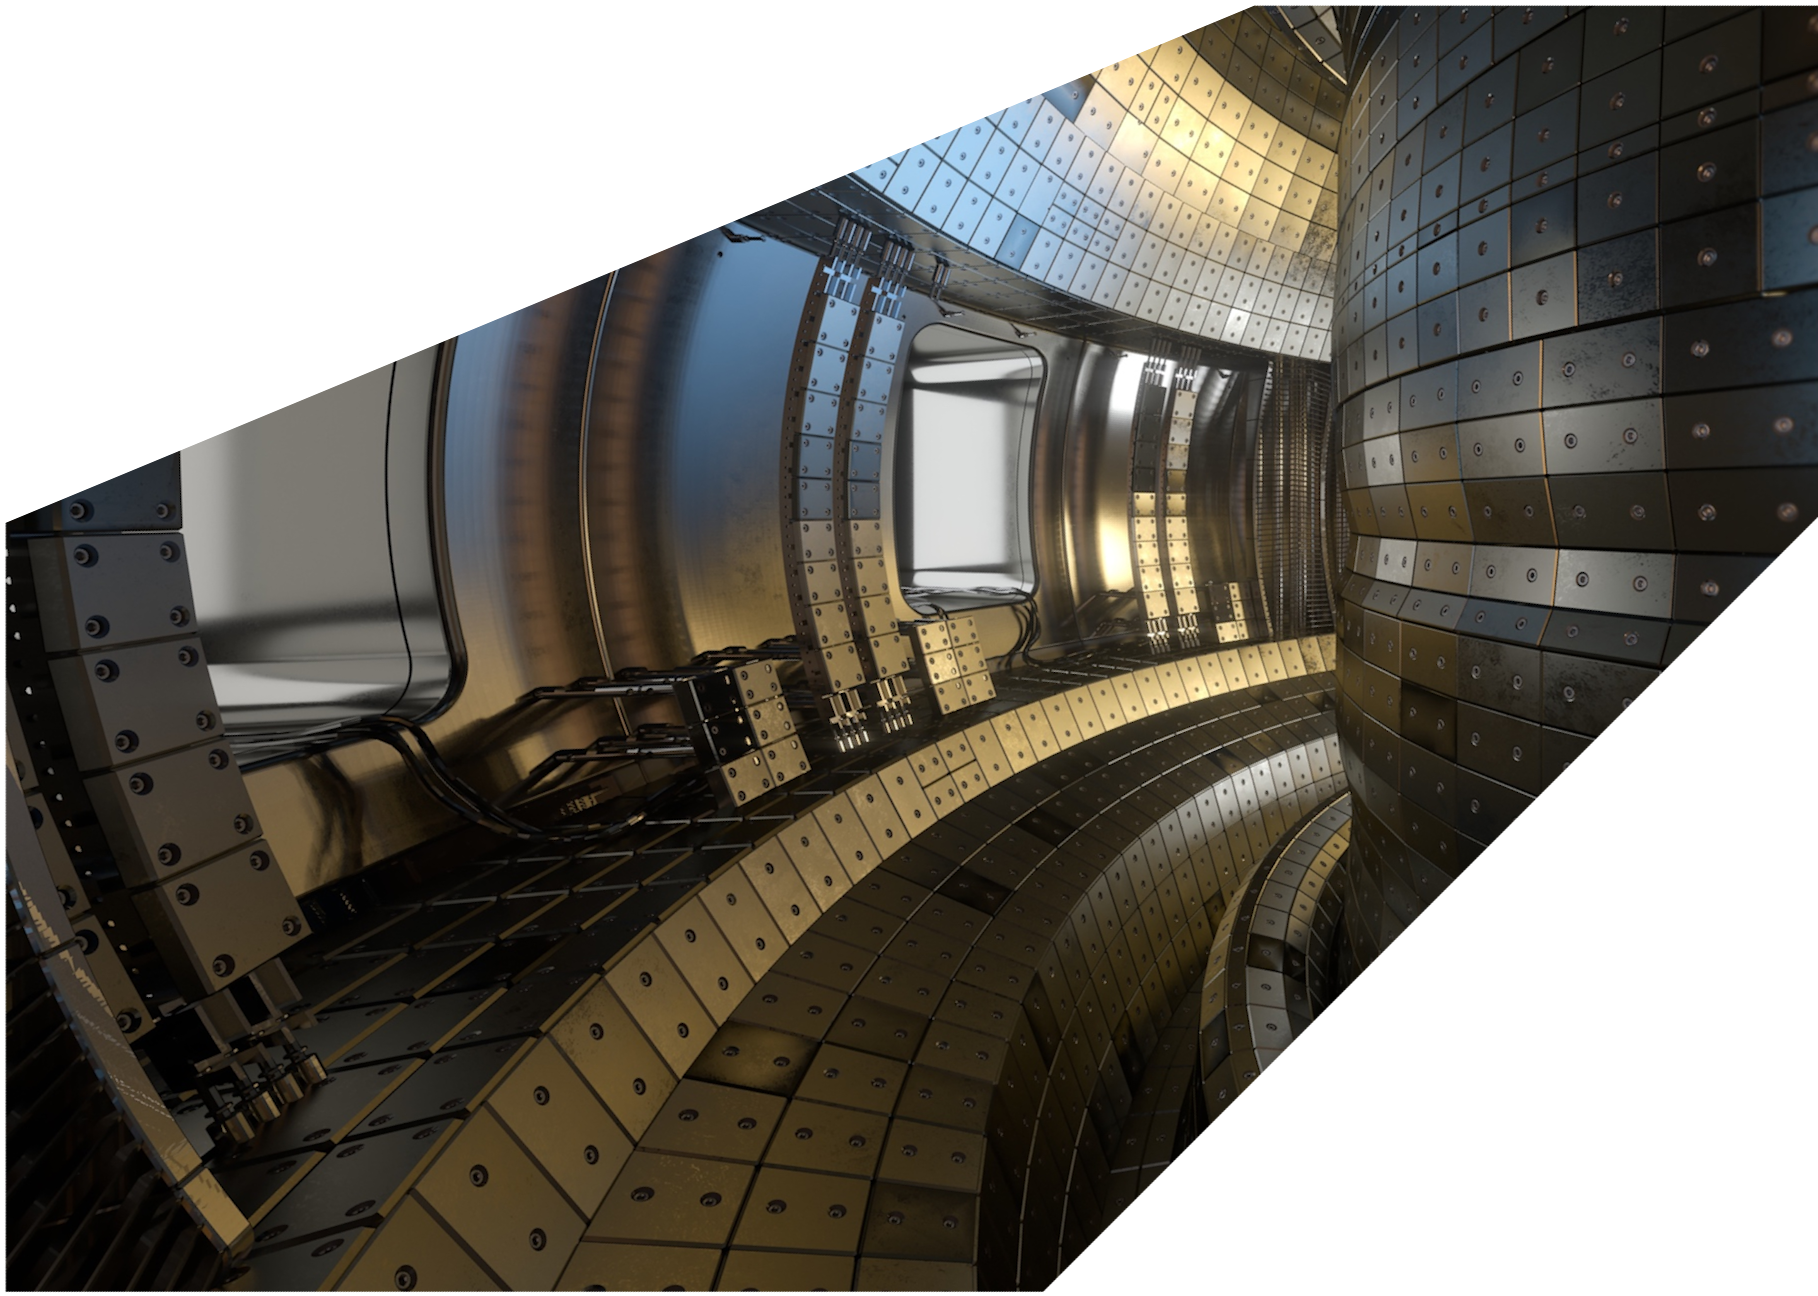
\includegraphics[width=0.9\textwidth]{../corpics/tokintcrop}}%<==omit
\end{titlepage}%<==omit

\hspace{-30mm}\begin{table}[h]
\sffamily
\begin{center}
\textbf{\textsf{UKAEA REFERENCE AND APPROVAL SHEET}}
\begin{tabular}{||p{5.7cm}|p{4.7cm}|p{5.0cm}||}
\hline
\hline
& Client Reference: &  \\
\hline
& UKAEA Reference: & \culhamshorttitle \\
& & \\
\hline
& Issue: & \culhamissueno \\
\hline
& Date: & \culhamdateb \\
\hline
\multicolumn{3}{||l||}{} \\
\multicolumn{3}{||l||}{Project Name: ExCALIBUR Fusion Modelling System} \\
\multicolumn{3}{||l||}{} \\
\hline
\end{tabular}
\begin{tabular}{||p{3.3cm}|p{4.6cm}|p{3.5cm}|p{3.6cm}||}
\hline
& Name and Department & Signature & Date \\
\hline
Prepared By: & \culhamauthora & N/A & \culhamdate \\
& \culhamauthorb & N/A & \culhamdate \\
& \culhamauthorc & N/A & \culhamdate \\
& \culhamauthor & N/A & \culhamdate \\
& & & \\
& BD & & \\
\hline
Reviewed By: & \culhamcontactname & 
\includegraphics[width=3.0cm]{../corpics/blanksign}& \culhamdatea \\
& & & \\
& Advanced Computing Dept. Manager & & \\
\hline
Approved By: & \culhamcontactname  & 
\includegraphics[width=3.0cm]{../corpics/blanksign} & \culhamdateb \\
& & & \\
& Advanced Computing Dept. Manager  & &\\
\hline
\hline
\end{tabular}
\end{center}
\end{table}


\clearpage
\section{Introduction}\label{sec:intro}
This report collates technical material used to inform the preparation of the call for 
procurement of support for Uncertainty Quantification~(UQ).
The work performed primarily consisted of collating material produced
internally~\cite{y2re241,y2re242,y2re251,y2re313}
and by external grantees at UCL~\cite{2047352_1-TN-01,2047352_2-TN-01}, plus
hands-on exploration of sampling techniques, the construction of surrogates and the study
of dimensionally reduced models.
The production of this call reflects the importance attributed to UQ in project \nep, so that 
the software produced should be capable of producing `actionable' results, that could form a significant
input to multi-million pound procurements.

It seems worthwhile to start by recapitulating the project
\nep \ requirements for UQ, insofar as they are currently understood. In particular, to
note a clear distinction between the experiments that \nep \ code needs to model, and the
outputs of the simulations themselves.  Relevant experiments are almost entirely medium-sized
and large tokamaks, where it seems that even the edge plasma has a temperature of
around~$10$\,eV~($10^5$\,K). The presence of magnetic fields of order $1-10$\,T, and
electric fields of around $10^4$\,Vm$^{-1}$ implies a hostile environment, subject further
to large electromagnetic transients not just at start-up and ramp-down of a discharge, but also caused by
plasma instabilities such as ELMs and sawteeth.  Most diagnostics struggle to achieve absolute
accuracies of $10$\,\%, although they usually detect the direction of smaller changes reliably.
Many are ``one-of-a-kind" so require careful interpretation, and all signals may have been subject to
filtering both at low and high frequencies, to remove  `spikes' and `drift'.
In comparison, signals from simulation are very `clean', but the simulation may lack
crucial realism, in that either important physical processes are not treated or 
if included, that the spatio-temporal discretisation may not be sufficiently fine to
represent them accurately.

%The Model  expt. - noisy, large unc. toks
%simulation - clean, level of detail controllable by mesh refinement, more detailed physics

Turning to the expected usage of the \nep \ software, this covers  both physics and engineering.
Both physicist and engineers are potentially interested in everything computed by the software, which is of course
likely to be an overwhelming amount of detail. A physicist is more likely to begin by
formulating simpler models and use the software to determine their appropriateness and accuracy,
an engineer probably more likely to use the output of simulation as a basis for producing simplified models.
An experimental physicist may be satisfied with qualitative accuracy, provided it is obtained
rapidly enough to help formulate the next experimental `shot' (eg.\ by indicating that more
or less gas input would be helpful), whereas a more theoretical
%counterpart may want a model useful for extrapolation to reactor parameters. An engineer
counterpart may want to quantify the difference between model predictions and experiment 
sufficiently well to help produce a more refined model. An engineer
seeking to design a reactor may be interested only in a relatively small number of
quantities of interest~(QoI) but which need to be determined more precisely, 
such as local maxima in time-averaged heat flux, whereas
other engineers may see edge code as forming a part of a digital twin, to be used to help control
operation of an actual tokamak device where accurate time-dependent modelling will also be critical.
%Users physicist -  formulate simpler models useful for extrapolation of geometry and parameter changes
%potentially interested in everything as extrapolation
%experimental physicist, qual accuracy OK for fuelling
%engineering design - few QoI, static
%digital twin (as part) - for operation and control, quant accuracy, time dep.
It is notable that most of the preceding requirements involve extrapolation,
from model to new features of an existing experiment or, in the design case, to more
extreme values of geometrical size, magnetic field etc. representing a fusion reactor
relative to existing experiments such as JET.
%Requirements - interpolation, to obtain sufficient data to perform to a given accuracy
%extrapolate - "to expt" and to new parameters

For the above it is therefore as Smith~\cite{smithUQ} describes (see also the \nep \
report~\cite[\S\,1]{y2re313}), important that UQ involves more than just clever sampling
to identify parameter sensitivities, and the standard definitions of ways of quantifying
these such as Sobol indices~\cite{y2re241}. In particular,
the production of surrogate models is within scope of UQ.
%sampling imp. for identifying important parameters
It is worth saying that in one sense even the most complex partial differential equation~(PDE) models of plasma are 
simply surrogates for experimental `reality'. The most detailed and least controversial
model of tokamak plasma consists in treating it as of order~$10^{20}$ or more particles evolving
under the influence of external and self-generated electromagnetic fields, but
this is of course not tractable even at the Exascale~\cite{Wa95a}, without very selective
sampling of the particles. Currently, particle models are seen as at best struggling to capture
edge plasma behaviour, with no certain likelihood of significant improvement, and 
in any event there is a separate calls that could cover research into particle sampling. The PDE models
attempt to capture the key physics of the plasma particles, viz.\ their appearance, motion,
interactions with other particles and eventual loss, as terms representing respectively
source, advection, diffusion and sinks in continuum models. Unfortunately, long mean free
paths~(\emph{mfp}s) mean that at least in some regions it is necessary explicitly to represent
phase-velocity dependence of plasma density, and the resulting basic 6-D dependence of 
fields (5-D if gyro-averaged models are used) stretches current and foreseen computing
facilities. In any event, above applications eg.\ preliminary design studies and operational control,
require models capable of evaluation within seconds or less, ie.\  surrogates for the
PDEs, expected to have lower spatial dimensionality (2-D or 1-D) or even as systems of 
ordinary differential equations~(ODEs).
%Surrogate. PDE solution as surrogate for expt/reality, advection, diffusion, sinks and sources.

Unfortunately for application to \nep, most surrogates have been designed for use as
interpolants. Nonetheless, interpolation is likely to be important at least within the software,
eg.\ to connect different models, and the book by de~Boor~\cite{deboor} has interesting
material relating to the use of splines in this context. In particular, de~Boor lists
theorems relating to the optimality of spline polynomial interpolation, so that there might be
wonder that any other form of interpolation is required. In fact, spline optimality is found only in 
the energy or least-squares norm, so there is anyway the possibility of fitting the data
with polynomial functions that have under- and over-shooting oscillations between sample
points (called nodes in spline jargon). Moreover, de~Boor illustrates the potential for dramatic failings
using what he refers to as the Titanium heat data set~\cite[Fig.\ XIII.1]{deboor}. The data is
a set of some~$50$ apparently regularly spaced samples of a function which is practically
flat except for one distinct `hump', rising to four times the value of the `plateau' over
c.\ $15$\,\% of the range. Since the interpolation is by a piecewise  ($5^{th}$ order polynomial)
the undershoot by greater than the maximum `hump' value is in many respects more impressive than
that exhibited in Boyd's book~\cite[Fig.\ 4.3]{boyd} as part of his demonstration of the Runge
phenomenon, ie.\ that polynomial interpolation at evenly spaced points may diverge. In both books,
the problem is identified as due to poor choice of sample points. de Boor~\cite[Fig.\ XIV.5]{deboor}
shows improved fitting if the number of samples in the plateau region of the \emph{Ti} heat data is reduced,
whereas Boyd points out that optimal $N^{th}$~order polynomial interpolation is achieved using
sample points that are the roots of the Chebychev
polynomial of degree~$(N+1)$, that cluster as close together as~$1/N^2$ near the end-points
of the sample region. In any event, for many interpolation purposes, it seems that polynomial spline
fitting with an order of three or so, is adequate \emph{provided} the nodes are chosen suitably. The cost
scales as the operation count  of a banded-diagonal matrix solver, so~$\mathcal{O}(N)$ where $N$~is the
number of points to be interpolated per dimension.
There are however strong proponents for the use of rational polynomial interpolation~\cite{stoerbulirsch}
and in particular radial basis function~\cite{fornbergflyer}. Wavelet bases~\cite{Fa15Wave} also
have their adherents, and special conditions such as periodicity or infinite domain mean that
respectively Fourier series and the Hermite basis are to be preferred. The Hermite basis is
employed in the Polynomial Chaos Expansion~(PCE), which is advocated by P.\ Coveney~et~al, see
the \nep\ report~\cite{2047352_1-TN-01}. % and special bases will not be discussed further

Accurate spline fitting requires a sufficient amount of data to enable best location of the
nodes, which, since they generally aim to use as few nodes as possible, is commonly unavailable
in the output of
highly expensive numerical calculations. This lack of data means also that interpolation using
Neural Networks~(NNs)  is mostly unsuitable, and motivates the use of Gaussian Processes~(GPs)
for interpolation despite their expense, that~$\mathcal{O}(N^3)$ of inverting a full matrix~\cite{y2re242}.
They come with the benefit of accompanying error bounds, and seem to be relatively stable when
used for extrapolation~\cite{Ch20priv}. They may be very effective in combination with a 
special basis produced by Principal Component Analysis~(PCA), \emph{aka} Proper Orthogonal Decomposition
or POD, see the \nep\ report~\cite{2047352_2-TN-01}. Moreover, S.~Guillas~\cite{Li17Dime} describes
a number of techniques which outperform PCA, in particular favouring a reproducing kernel
approach to estimating derivatives needed to optimise the basis. This is coupled with
a sequential approach to selecting sample points.
Indeed, choosing sample points appropriately is still a major issue for GPs, which P.~Challenor (private
communication) has explored extensively and favours `Leave One Out'~(LOO).

% as interpolant (1) polynomial spline, GP, NN.
%limitations of spline, GP and NN in table/appendix.
%De Boor for spline, Ti heat data XIII.1 - Gibbs like phena - but XIV.5 shows OK if get nodes
%in right place
Nonetheless, given the general need for extrapolation, it is desirable to incorporate as much
physical knowledge as possible into the surrogate model. The hopes are that the parameters
of the surrogate are either invariant under the extrapolation, or that they have well-determined
scaling properties, and that all important physical processes have been identified.
The parameters of the surrogate may then be fitted using existing data from
experiment and/or simulation as described above.
The surrogate may need to be space and/or time dependent as required by the
user and application. Of course, such surrogates can be very useful for interpolation also.
Worthy of particular mention is Model Order Reduction~\cite{y2re251}, which for linear and some nonlinear
problems, offers reliable estimates of error in interpolating Quantities of Interest~(QoI),
hence likely to be particularly useful for the design engineer.

The body of the current document consists of hands-on exploration of sampling techniques
in \Sec{bout}, the construction of surrogates by Gaussian Processes in \Sec{nektar} and
of surrogates consisting of dimensionally reduced models in \Sec{dimred}.
The implications for the call are summarised in \Sec{summ}.
%ed
\clearpage
\section{BOUT++}\label{sec:bout}
\subsection{BOUT++}\label{sec:bout}


BOUT++ \cite{bout431,boutwebsite,boutrepo} describes itself as
\begin{quote}
a framework for writing fluid and plasma simulations in curvilinear geometry. The design is modular, with a variety of numerical methods and time-integration solvers available that can be chosen at runtime. BOUT++ is primarily designed and tested with reduced plasma fluid models in mind, but it can evolve any number of equations, with equations appearing in a readable form. The code is opensource, licensed under the LGPL, and is available from https://github.com/boutproject/BOUT-dev
\end{quote}

\paragraph{Framework}

BOUT++ is a multi-block finite difference / volume PDE solver written in C++, with parallelisation using MPI and/or OpenMP.
GPU acceleration is under development.
There are optional dependencies on a variety of third-party libraries such as FFTW, SUNDIALS, PETSc, SLEPc. I/O is via netCDF or HDF5. 

The core of BOUT++ is a library of functions relevant to plasma simulation in 3-D curvilinear geometry, such as differential operators, definitions of tokamak domains and magnetic geometries (e.g. single/double null), and common boundary conditions. 
BOUT++ also provides routines for integrating equations in time and for inverting elliptic operators.

As a library, BOUT++ does \emph{not} specify the equations to be solved.
These are specified by the user in defining their ``PhysicsModel'', a class that provides ``init'' (initialization) and ``rhs'' (right-hand side) functions.
The class is then passed to BOUT++, that is, the user cedes control of the workflow to the library.

In addition to the core library, the BOUT++ project also provides Python utilities for grid generation, post-processing and plotting in tokamak geometries.

\paragraph{Domain-specific language}
The BOUT++ library routines provide a domain-specific language (DSL), allowing the user to specify equation systems in a human-readable fashion.
For example, the wave equation (for amplitude $f$ and velocity $g$ and unit wavespeed) may be written in the user's physics model as
\begin{align*}
  \mathtt{ddt(f) = Grad\_par(g);}\\
  \mathtt{ddt(g) = Grad\_par(f);}
\end{align*}
This allows physics models to be implemented in BOUT++ with minimal effort, allowing rapid prototyping.
It also means there is a very low bar to entry for new users/non-programmers, and physics models may be implemented with no knowledge of the underlying numerics -- for better or worse!

\paragraph{Performance}
BOUT++ is a versatile framework that may be run across the spectrum of computing system sizes, from laptops to large HPC systems.
BOUT++ is currently deployed on Archer (UK Tier-1) and Marconi (Tier-0), among others, and scales to ${\cal O}(1000)$ cores for typical problem sizes.

Two of the three dimensions are parallelized with MPI, while all dimensions are parallelized with OpenMP (recasting the 3-D arrays local to an MPI rank as a flat vector).
The MPI parallelization in one of the dimensions and the OpenMP parallelization were retrofitted -- the anisotropy of plasma in strong magnetic fields meant that in early simulations the resolution used in all-but-one of the dimensions was not sufficiently large to merit parallelization.

\paragraph{Software sustainability and community}
BOUT++ is freely available via the public Github repository \cite{boutrepo}, and is licensed under the LGPL. Development is done in public, with regular feedback from community members.
%
BOUT++ uses a development model similar to gitflow, with a stable \texttt{master} branch and a development \texttt{next} branch. \texttt{next} forms the basis for major and minor releases, so new features are introduced into \texttt{next}, while bugfixes are introduced into both \texttt{master} and \texttt{next}.
Both these branches are protected, and new code only enters via a pull request, which requires code review and approval from a maintainer before being merged.
Travis CI is used to automatically run a comprehensive suite of both unit and system (integrated) tests on every push to the Github repository. Creation and update of pull requests triggers additional tests. Several build configurations are tested, including optimised builds, different compilers and Linux distributions, and linking against various optional third party libraries.

New releases are recorded on Zenodo, allowing each release to have a citable Digital Object Identifier (DOI).
Having a DOI for each version is important for reproducibility of scientific results, but producing an accompanying paper for releases simply to obtain a DOI may be an incommensurate amount of work, or not deemed of sufficient interest to be publishable.
Reproducibility is further aided by the output of each run recording the git commit hash and the state of the repository (``clean'' or ``modified'').

Documentation is automatically built from doxygen comments in the source code and hosted online at ReadTheDocs \cite{boutreadthedocs}, while bug reports and community feedback can be done via the Github issue tracker or the BOUT++ Slack workspace.

Hands-on training led by the maintainers is provided for new users at annual workshops, where users can also present their research and discuss new and future code development and features. Research and code development can also be presented at the monthly user meetings, held via video conference.

\paragraph{Summary}

BOUT++ is a versatile, easy-to-use and reasonably-performative framework.
It successfully implements a ``separation of concerns'' between the roles of user and developer.
For users, the DSL allows models to be written in human-readable form, with simple access to complicated geometry-dependent operators.
Different numerical methods for discretization and time-integration may be selected at run-time.
This means there is a low barrier to entry for prototyping models, and for running simulations on Tier-0/Tier-1 HPC systems.
For developers, the source code is freely available on the repository, along with contribution guidelines.
There is also an active community of developers around the repository, Slack channel and BOUT++ User Group meetings.

Not all features of BOUT++ are appropriate for ExCALIBUR projects however.
BOUT++ emphasizes flexibility rather than performance. 
One example of this is in the domain specific language where BOUT++ favours a clear interface for the DSL, over optimal performance for any one set of systems.
Requiring that operators (such as \texttt{Grad\_par(g)} above) are independent objects means that the right-hand side functions are concatenations of objects, each being relatively small kernels of work. 
Joining these into a single loop would require introducing a global index and an outer loop, so operators would be written \texttt{Grad\_par(g)[i]}.
While this could be circumvented with code generation techniques, this has not yet been implemented, and BOUT++ developers favour the cleaner interface to raw performance.

There is also an issue with political control of the users' physics models. 
The library nature of BOUT++ allows users to develop sophisticated models (e.g. STORM (from CCFE), Hermes and SD1D (from the University of York), plus other models from other individuals/institutions), which themselves require infrastructure like repositories, testing and contribution guidelines. 
These models have varying degrees of independence from the core BOUT++ framework.  
Hermes and SD1D are developed by the core BOUT++ developers; STORM is developed in collaboration with BOUT++ developers; in contrast, the source code for physics modules belonging to other institutions are not usually available to BOUT++ core developers.
    Yet all of these may be presented in papers or at conferences as being ``BOUT++''.
    This is a reputational risk to the BOUT++ project.
    It has been mitigated to some extent by bringing some physics modules into the main repository and testing them, and by endeavouring to collaborate as widely as possible.

\clearpage
\section{Nektar++}\label{sec:nektar}


Nektar++ \cite{Mo20Nekt, nektarwebsite} is a framework for solving partial differential equations (PDEs) using the spectral / hp-element method.  
The software contains several different solvers targeting canonical problems in fluid mechanics.  
It is possible to extend the framework by adding new domain-specific solvers; this currently involves low-level coding as there is no DSL.  
Nektar++ is being used in Project \nep\ as the framework for the higher-order solution of fluid equations and currently is being extended to handle plasma fluids.  Data is extracted from Nektar++ simulations by means of \emph{filters} and written to text-based output files.

A small team from UKAEA 
%(Ed Threlfall and Will Saunders) 
attended the three VECMAtk hackathons in Spring 2021.
The goal of the hackathon work was to create the software framework to enable
Nektar++ to use VECMAtk,
and to develop workflows for uncertainty quantification and the creation of
surrogate models.
%The code produced at the hackathons is available in the repository \cite{nektar_vecma_repo}.

\subsection{Software Infrastructure}

The VECMA toolkit wraps around an individual Nektar++ solver to provide non-intrusive UQ (only non-coupled workflows are considered here).  
The toolkit interacts with Nektar++ via the inputs and outputs of the latter, through respectively an \emph{encoder} and a \emph{decoder}; 
these objects can be interchanged to enable different workflows (for example, the relevant quantities of interest (QoIs) are parsed in the decoder). 

\subsection{Uncertainty Quantification}

The initial test problem used the incompressible Navier-Stokes solver of Nektar++ to simulate classical convection: 
a two-dimensional fluid-filled slot with vertical walls maintained at different temperatures; starting with an initial uniform temperature gradient from the hot side to the cold side, the system is time-evolved until a steady state is reached.  
Warmer fluid is subject to an upward buoyancy force, leading to a steady convective cell solution with fluid travelling up the hot side and down the cold one.

In dimensionless form, the equations for fluid velocity $\bf{u}$, temperature $T$ and pressure $p$ are

\begin{eqnarray}
\frac{1}{Pr} \left ( \frac{\partial \bf u}{\partial t} + {\bf u} \cdot \nabla {\bf u} \right ) &=& - \nabla p + Ra \; T \; \hat{{\bf y}} + \nabla^2 {\bf u}\\
\left ( \frac{\partial T}{\partial t} + {\bf u} \cdot \nabla T \right ) &=& \nabla^2 T\\
\nabla \cdot {\bf u} &=& 0.
\end{eqnarray}

Here, the Rayleigh number $Ra$ and the Prandtl number $Pr$ are the governing parameters and are taken to be subject to uncertainty. 

%The QoIs are the Nusselt number, the dimensionless heat flux across the cavity (normalized to the $Ra=0$ solution, which corresponds to the initial data)

%\begin{equation}
%Nu = -\frac{1}{2H} \int_0^H \nabla_x T(x_0,z)+\nabla_x T(x_1,z) dz.
%Nu = \frac{ \int_0^H -\nabla_x T(x_0,y)+\nabla_x T(x_1,y) dy }{ \int_0^H -\nabla_x T(x_0,y)+\nabla_x T(x_1,y) dy \rvert_{Ra=0}}
%\end{equation}

%and also the temperature profile across a horizontal line half-way up the cavity.

The Nektar++ simulations were designed so as to run quickly on a single desktop computer.  
Computational parameters governing accuracy were chosen to give plausible results without detailed analysis of convergence.

\subsubsection{Polynomial chaos expansion}

A square slot was used as a first example; the results follow closely the original investigation in \cite{El65Nume}.  
An example temperature profile over the full domain can be see in Figure \ref{fig:tempfield}.

\begin{figure}[tbp]
\begin{centering}
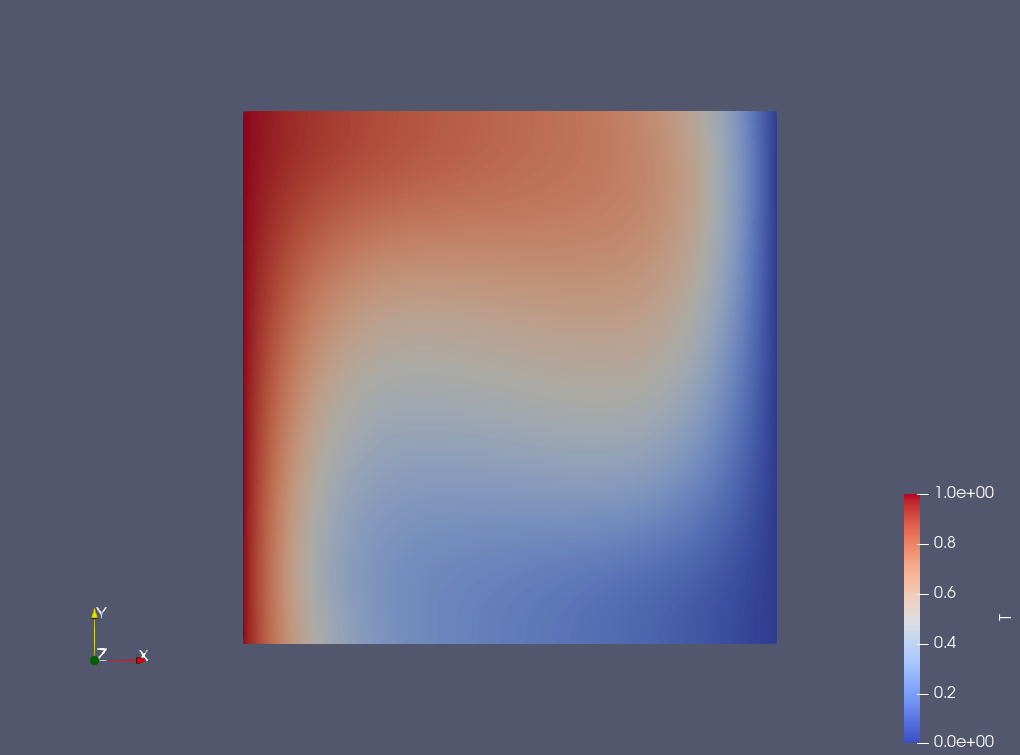
\includegraphics[width=0.5\textwidth]{laminar.png}
\caption{\small Steady-state colour map of dimensionless temperature for $Ra=10^4$, $Pr=1.0$.  The left side is maintained at a temperature one unit higher than the right and a convective cell carries fluid in a clockwise circulation.
\label{fig:tempfield}
}
\par
\end{centering}
\end{figure}

The QoI was the temperature profile $T(x)$ evaluated half-way up the slot, parsed via the decoder \texttt{SlicedHisDecoder} from data extracted using the Nektar++ \texttt{HistoryPoints} filter to record field values at chosen sample points.  %Again, a decoder (\texttt{SlicedHisDecoder}) parses a text file output by Nektar++ and extracts the QoI.
Note that the sample points cannot lie on the vertical boundaries, as the Dirichlet boundary condition enforces constant temperature values there, which causes the analysis to fail (a singular matrix error is reported by VECMA).  
$Pr$ was taken to be in the range $1-10$ (values typical for the gases and liquids commonly investigated in the literature), with a uniform distribution.  
$Ra$ was taken to be in the range $1.0\times 10^4 - 3.2 \times 10^4$ (values consistent with a laminar convective steady state), with a log-uniform distribution.

The polynomial chaos expansion (PCE) produces a fit to the sampled QoI data using a sum over orthogonal polynomials in the input variables, where the orthogonality is defined using the input probability distributions as the measure and the fit is performed by either spectral projection or linear regression.  
The polynomial chaos analysis of EasyVVUQ provides the mean, variance, and standard deviation of the outputs and also the minimum, maximum, median and the $1^{st}$, $10^{th}$, $90^{th}$, and $99^{th}$ percentiles (a useful \texttt{supported\_stats()} routine lists the available statistics).  
Some of these quantities are shown in Figure \ref{fig:temp_profile}, which was generated using a fifth-order PCE.  
Also shown are the first Sobol indices, which show correctly that the uncertainty in the output is dominated by the sensitivity to~$Ra$ in this case; in the regime in question, the effect of varying $Pr$ is small.

\begin{figure}[tbp]
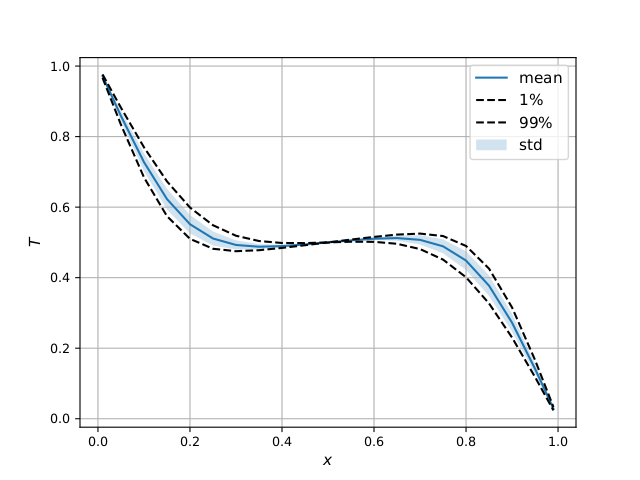
\includegraphics[width=0.5\textwidth]{T_vs_x_mean_ci_nektar.png}
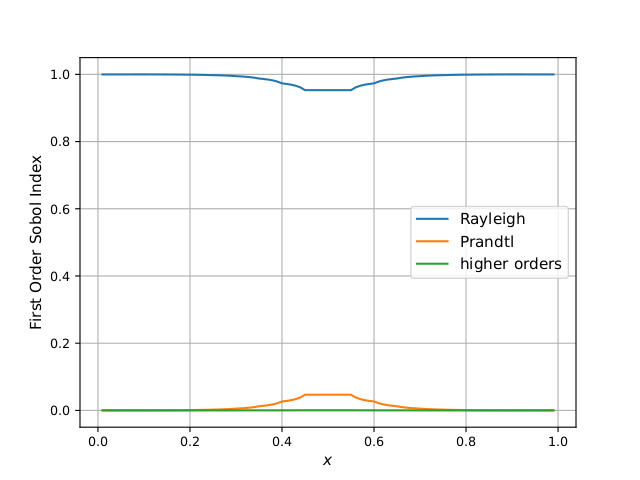
\includegraphics[width=0.5\textwidth]{T_vs_x_sobols_nektar.png}
\caption{%
Mean and confidence intervals (left) and first Sobol indices (right) as a function of position
for the central temperature profile $T(x)$ fitted by a polynomial chaos expansion.  Note that the uncertainty tends to zero in regions where the temperature is 
either fixed (end points) or is constrained by symmetry (centre).  
\label{fig:temp_profile}
}
\end{figure}

\subsubsection{Stochastic collocation}

Stochastic collocation (SC) creates a representation of the QoIs that is exact at the sample points; the solution is a linear combination of sample-point values multiplying Lagrange polynomials at those points.  
The stochastic collocation analysis of EasyVVUQ provides the mean, variance and standard deviation of the outputs.  
The set of available statistics is smaller than for the PCE, but the method is more efficient (as explained earlier in this report).  
The decoder used in the preceding section is switchable between PCE and SC.

\subsection{Surrogate models}

Note that, although it concerns surrogate models, the work in this subsection used EasyVVUQ and not EasySurrogate.

\subsubsection{Polynomial chaos expansion and stochastic collocation}\label{sec:pceasc}

Either of the orthogonal polynomial fit constructed in the polynomial chaos expansion or the Lagrange polynomial fit constructed in the stochastic collocation method can serve as a computationally-inexpensive surrogate for the full model.  
As an example, PCE and SC surrogates for the Nusselt number $Nu$ as a function of $Ra$ and $Pr$ were constructed.  $Nu$ is the dimensionless heat flux across the cavity, normalized to the $Ra=0$ no-convection solution, calculated as

\begin{equation}
%Nu = -\frac{1}{2H} \int_0^H \nabla_x T(x_0,z)+\nabla_x T(x_1,z) dz.
Nu = \frac{ \int_0^H \partial_x T(x_0,y)+\partial_x T(x_1,y) dy }{ \int_0^H \partial_x T(x_0,y)+\partial_x T(x_1,y) dy \rvert_{Ra=0}} \; .
\end{equation}
where $\partial_x$ denotes partial derivative with respect to coordinate~$x$.

The Nusselt number was extracted using a customized filter in Nektar++ and the output file was parsed by a decoder (\texttt{HeatFluxDecoder}) using a simple text processing routine.  
An illustration of the SC and PCE fits (both using fifth-order polynomial expansions) for the simple case of Nusselt number as a function of the Rayleigh number ($Pr=1$) is shown in Figure \ref{fig:nektar_surrogate}.  
The Nusselt number is seen to follow a typical power-law curve.

\begin{figure}[tbp]
\begin{centering}
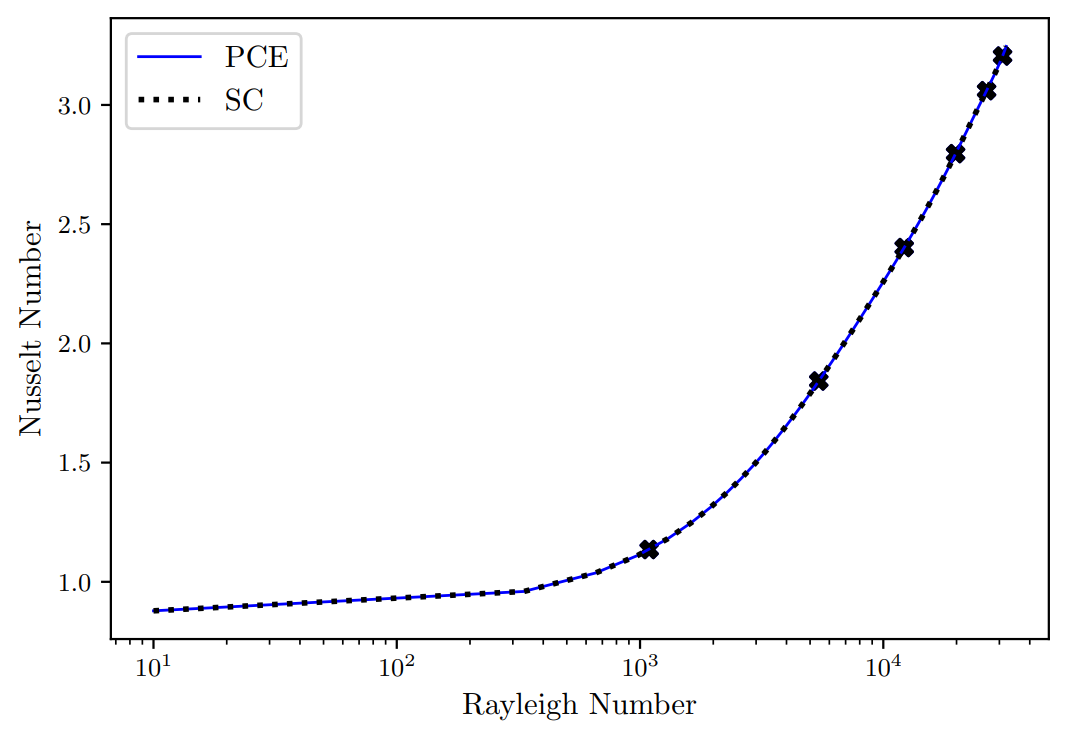
\includegraphics[width=0.5\textwidth]{nektar_surrogate.png}
\caption{\small Polynomial chaos and stochastic collocation surrogates for Nusselt number as a function of Rayleigh number, for Prandtl number $1.0$.
\label{fig:nektar_surrogate}
}
\par
\end{centering}
\end{figure}

\subsubsection{Gaussian process surrogate}

A different set-up, though again using the Nektar++ incompressible Navier-Stokes solver, was used as an initial exploration of the Gaussian process surrogate capability in EasyVVUQ; 
this was a slot $10$ units high and $1$ wide, operating at larger Rayleigh numbers where the flow exhibits a boundary-layer instability with waves moving up the hot wall and down the cold one (illustrated in Figure \ref{fig:wallwavesetc}).  
This gave interesting time series for the maximum temperature near the affected parts of the walls (the lower part of the cold wall was used) and the position of the hottest point.  
These QoIs are of interest in fusion applications as they characterize the hot spots on the wall of a reactor containing hot plasma.  
The time series were extracted over a chosen time window using a customized filter in Nektar++; 
the simulation runs were performed once and the decoder (\texttt{HotSpotDecoder}) was given the ability to read stored simulation data in order to avoid repeating calculations.
In view of the weak dependence on the parameter $Pr$, only the parameter $Ra$ was varied in this activity (values in the range $10^5-10^7$ were used).  
A kernel with zero mean and a Mat\'ern covariance with parameters $\nu=3/2$ and scale $10^7$ were used.

\begin{figure}[tbp]
\begin{centering}

\includegraphics[height=0.6\textheight]{wall_waves.png}\\
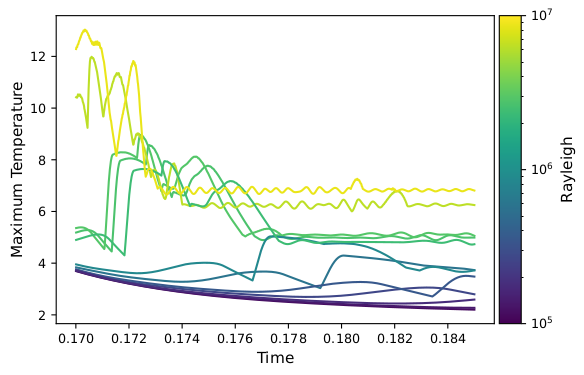
\includegraphics[width=0.4\textwidth]{gp_observed_max_temp.png}
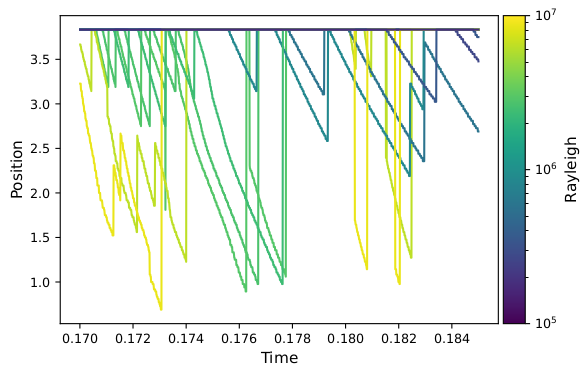
\includegraphics[width=0.4\textwidth]{gp_observed_position.png}
\caption{\small Boundary-layer instability at the cold wall for $Ra=2.3 \times 10^8$ (top). 
The maximum temperature on this part of the wall and also the position of the hottest point are shown as time series (respectively left and right below).
\label{fig:wallwavesetc}
}
\par
\end{centering}
\end{figure}

This investigation was an attempt at finding a surrogate for computations that are more demanding than the laminar convection ones in the preceding section and also concerned a system that exhibits deterministic chaos.
The time series data used to train the Gaussian process is shown in Figure \ref{fig:wallwavesetc}.  
Note that for $Ra$ sufficiently large for the instability to form, temperature maxima enter from the top of the monitored section and proceed downwards until usurped by the next wave.  
For smaller values of $Ra$, the system is quiescent and the time series eventually become constant.
Some sample evaluations of the Gaussian process surrogate away from the sample points can be seen in Figure \ref{fig:GPoutputs}.  It can be seen that the surrogate correctly reproduces the more active nature of the time series for larger values of $Ra$.

\begin{figure}[tbp]
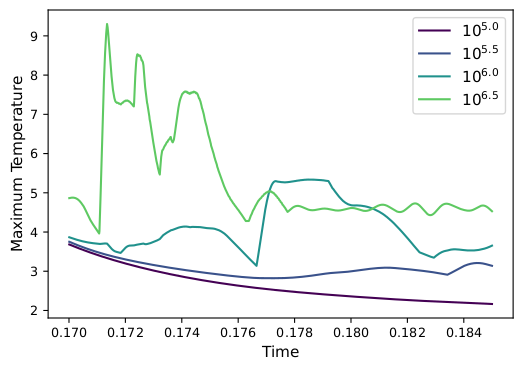
\includegraphics[width=0.5\textwidth]{gp_sample_max_temp.png}
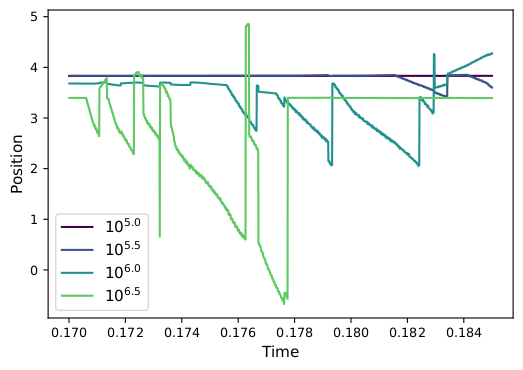
\includegraphics[width=0.5\textwidth]{gp_sample_position.png}
\caption{%
Output of the Gaussian process surrogates for the maximum temperature and the position of the hottest point evaluated at positions away from the sample parameter values.  
\label{fig:GPoutputs}
}
\end{figure}









\clearpage
\section{Dimensionally reduced models}\label{sec:dimred}
\subsection{Boltzmann Equation}\label{sec:boltz}
One suggestive example of the production of a surrogate is the reduction of the Boltzmann equation to 
the equations of fluid dynamics. The model is a combination of Lie derivative and solenoidal constraints
\begin{eqnarray}\label{eq:lie}
 \frac{\partial f}{\partial t} + u_x  \frac{\partial f}{\partial x} + u_y  \frac{\partial f}{\partial y} &=& S\\
 \frac{\partial u_x}{\partial x} +  \frac{\partial u_y}{\partial y} &=& 0 \label{eq:sol}
\end{eqnarray}
where $f(x,y,t)$ is the phase space density as a function of time~$t$,
$u_x$ is the flow in position space~$x$, and $u_y$ is the flow in velocity space~$y$.
Collision and other source terms are represented as~$S(x,y,t)$.
For simplicity, it is assumed that position and velocity space are each~1-D. In more conventional
notation where $v$ is the velocity space coordinate and $a$ the acceleration experienced by
a particle, then  $y \leftrightarrow v$, $u_x=v$  and $u_y = a$.

Integrating \Eq{lie} over velocity space, ie.\ forming $\int \cdot dy$ leads to
\begin{equation}\label{eq:nconkin}
 \frac{\partial n}{\partial t}  +  \frac{\partial}{\partial x} \int u_x f dy- \int \frac{\partial u_x}{\partial x} f dy+  \frac{\partial}{\partial y} \int u_y f dy- \int \frac{\partial u_y}{\partial y} f dy= \int S dy
\end{equation}
upon using 
\begin{equation}
u_x  \frac{\partial f}{\partial x} =  \frac{\partial  (u_x f)}{\partial x} -  f  \frac{\partial u_x}{\partial x}
\end{equation}
and introducing
\begin{equation}
n = \int f dy
\end{equation}
Using \Eq{sol} so that two terms cancel, \Eq{nconkin} becomes
\begin{equation}\label{eq:nconsimp}
 \frac{\partial n}{\partial t}  +  \frac{\partial}{\partial x} \int u_x f dy+  [  u_y f ]_{\pm y_b} = \int S dy
\end{equation}
If $f$ and/or $u_y$ vanish(es) at the boundaries of the velocity domain $y=\pm y_b$, the third term is zero.
Suppose there is a mean flow, ie.\ that $u_x$ may be written 
\begin{equation}\label{eq:usplit}
u_x = U(x) + \tilde{u} (x,y)
\end{equation}
such that 
\begin{equation}\label{eq:zeromean}
\int \tilde{u} f dy=0
\end{equation}
and thus
\begin{equation}\label{eq:usplitf}
\int u_x f dy  = n U
\end{equation}
then substituting \Eq{usplit} in the second term of \Eq{nconsimp} results  in
\begin{equation}\label{eq:masscon}
 \frac{\partial n}{\partial t}  +  \frac{\partial  nU}{\partial x} = S_0
\end{equation}
which is recognised as the fluid dynamical equation of mass conservation with
source~$S_0(x)= \int S dy-[  u_y f ]_{\pm y_b}$.

To obtain the momentum conservation equation from \Eq{lie}, form $\int \cdot u_x dy$ and rearrange
$f$-derivative terms, leading to
\begin{equation}\label{eq:momconkin}
 \frac{\partial  nU}{\partial t}  +  \frac{\partial}{\partial x} \int u_x^2 f dy- \int \frac{\partial u_x^2}{\partial x} f dy+  \frac{\partial}{\partial y} \int u_x u_y f dy- \int  \frac{\partial (u_x u_y)}{\partial y} f dy= \int S u_x dy
\end{equation}
Using 
\begin{equation}
\frac{\partial (u_x u_y)}{\partial y} =  u_x \frac{\partial  u_y}{\partial y} +   \frac{\partial u_x}{\partial y} u_y = -  u_x  \frac{\partial  u_x}{\partial x} +   \frac{\partial u_x}{\partial y} u_y
\end{equation}
(the second manipulation using \Eq{sol}), \Eq{momconkin} gives
\begin{equation}\label{eq:momcons2}
\frac{\partial  nU}{\partial t}  +  \frac{\partial}{\partial x} \int u_x^2 f dy-  \int u_x  \frac{\partial u_x}{\partial x} f dy+ [ u_x u_y f ]_{\pm y_b}  - \int u_y  \frac{\partial u_x}{\partial y} f dy= \int S u_x dy
\end{equation}
Writing $u_x =U(x,t) + \tilde{u}$, the second term expands to
\begin{equation}
 \frac{\partial}{\partial x} ( U^2 \int f dy) + 2  \frac{\partial}{\partial x} (U \int \tilde{u} f dy) +  \frac{\partial}{\partial x} \int \tilde{u}^2 f dy
\end{equation}
which since $\int \tilde{u} f dy=0$, reduces to 
\begin{equation}\label{eq:term2}
  \frac{\partial  (n U^2)}{\partial x}  +   \frac{\partial}{\partial x} \int \tilde{u}^2 f dy
\end{equation}
The third term in \Eq{momcons2} is zero provided
\begin{equation}
 \frac{\partial u_x}{\partial x} = 0
\end{equation}
Indeed if $u_x=y$, then upon  introducing
\begin{equation}
p= \int \tilde{u}^2 f dy
\end{equation}
and
\begin{equation}
G= \int u_y f dy = \int a f dy
\end{equation}
there results the fluid dynamical equation of momentum conservation with momentum source $S_1(x)= \int S u_x dy-[ u_x u_y f ]_{\pm y_b}$,
namely:
\begin{equation}\label{eq:momcon}
 \frac{\partial nU}{\partial t}  +  \frac{\partial  nU^2}{\partial x} = -  \frac{\partial p}{\partial x} + G + S_1
\end{equation}

It may be helpful to note that the third term in \Eq{momcons2} expands to
\begin{equation}\label{eq:3rd}
- (n U  \frac{\partial U}{\partial x} + U \int \frac{\partial \tilde{u}}{\partial x} f dy+    \int \tilde{u} \frac{\partial \tilde{u}}{\partial x} f dy)
\end{equation}
where \Eq{zeromean}  has been used to zero one term.

%
%\begin{equation}
%\int u_x  \frac{\partial u_x}{\partial x} f dy= U  \frac{\partial U}{\partial x} \int f dy+ U \int \frac{\partial \tilde{u}}{\partial x} f dy+ \frac{\partial U}{\partial x} \int \tilde{u} f dy+  \frac{1}{2} \int \frac{\partial \tilde{u}^2}{\partial x} f dy
%\end{equation}
%\begin{eqnarray}\label{eq:terms}
%\mbox{Second term}&:&\frac{\partial}{\partial x} ( U^2 \int f dy) + 2  \frac{\partial}{\partial x} (U \int \tilde{u} f dy) +  \frac{\partial}{\partial x} \int \tilde{u}^2 f dy \\
%\mbox{Third term}&:&- (U  \frac{\partial U}{\partial x} \int f dy+ U \int \frac{\partial \tilde{u}}{\partial x} f dy+   \frac{1}{2} \int \frac{ \partial \tilde{u}^2}{\partial x} f dy) \label{eq:3rd}
%\end{eqnarray}

\subsection{Lie Derivative Surrogate}\label{sec:lied}

In the absence of sources \Eq{lie} may be written for a flow
${\bf u}$ in any number of dimensions as
\begin{equation}\label{eq:lief}
\frac{\partial f}{\partial t} + {\bf u}.\nabla f =0
\end{equation}
To proceed to derive a widely used class of surrogate for models involving
Lie derivatives,  it is helpful to run over a small amount of mathematics.
The streamlines of a vector field such as~${\bf u}$ by definition satisfy
\begin{equation}\label{eq:strml}
\frac{d {\bf x}}{ds}={\bf u }({\bf x})
\end{equation}
where ${\bf x}(s)$ is the streamline parameterised by~$s$, and where often
$s$ is chosen to be arc-length along the curve.
Hence substituting \Eq{strml} in ${\bf u}.\nabla f$ gives the Lie derivative
as $d f/d s$ which illustrates its
coordinate independence, since $s$ is an almost arbitrary label.
Further,  substituting \Eq{strml} in \Eq{lief} gives
\begin{equation}\label{eq:scal1}
\frac{\partial f}{\partial t} +  \frac{\partial f}{\partial s} =0
\end{equation}
where now $f(s,t)$. \Eq{scal1} is well-known to have the exact solution
$f=F(t-s)$ for arbitrary scalar functions of a single variable~$F$.
In realistic applications, $S\neq0$, but  the property that $f$ is a function only of arclength
(and time) survives, so that the physics of sources and sinks may be dealt with by a surrogate
which has only one space dimension supposing the streamlines are known.
Moreover, in the plasma context, the main flow may often be directed along
lines of magnetic field~${\bf B}$, so that exactly the same statements could be made 
replacing streamline with fieldline.

Now, \Eq{momcon} can be expressed in Lie derivative form by eliminating 
$\frac{\partial n}{\partial t}$ using \Eq{masscon}, and division by~$n$, giving
\begin{equation}\label{eq:liemom}
 \frac{\partial U}{\partial t}  +  U \frac{\partial  U}{\partial x} = -\frac{1}{n} \left(  \frac{\partial p}{\partial x} + G + S_1 - U S_0 \right)
\end{equation}
Thus provided ${\bf u}$ is expressed in Cartesians, each component separately obeys an
equation of the form \Eq{lief} and similar remarks apply. There is also~\cite{Wa13a}  a (pseudo-)vector
Lie formulation for~${\bf B}$ and the vorticity~${\bf \nabla}\times{\bf u}$ which can lead to
similar simplifications and potential surrogates.


\subsection{Surrogates for advection}\label{sec:adv}

\Eqs{lie}{sol} combine to give an equation identical to that for mass conservation in 2-D, namely
\begin{equation}\label{eq:masscon2d}
\frac{\partial f}{\partial t} +  \frac{\partial (u_x f) }{\partial x} + \frac{\partial (u_y f)}{\partial y} = S
\end{equation}
where now $f(x,y,t)$ is the fluid density as a function of time~$t$,
and $u_x$ and $u_y$  are components of the flow~${\bf u }$.
Source terms may still be represented as~$S(x,y,t)$, 
collision terms may be represented as a further contribution to~$S(x,y,t)$, of form
\begin{equation}\label{eq:diffus}
S_d=\frac{\partial}{\partial x} \left( \kappa_{xx} \frac{\partial f}{\partial x} +
\kappa_{xy} \frac{\partial f}{\partial y} \right) +
\frac{\partial}{\partial y} \left( \kappa_{yx} \frac{\partial f}{\partial x} +
\kappa_{yy} \frac{\partial f}{\partial y} \right)
\end{equation}
The above 2-D expressions should be sufficient for understanding how to deal with many
situations involving advection, diffusion and sources, which are more generally formulated as
\begin{equation}\label{eq:AD}
\frac{\partial f}{\partial t} + \nabla \cdot ({\bf u} f-\kappa \nabla f) =S
\end{equation}
for tensor diffusion coefficient~$\kappa$.

Analogous to \Sec{boltz}, integrating \Eq{masscon2d} over coordinate~$y$,
ie.\ forming $\int \cdot dy$ leads to
\begin{equation}\label{eq:masscon1d}
 \frac{\partial \int f dy}{\partial t}  +  \frac{\partial}{\partial x} \int u_x f dy+  [  u_y f ]_{y=\pm y_b} = \int S dy
\end{equation}
There is then a simplification to a 1-D surrogate upon supposing
that as in \Sec{boltz} $u_x$ may be written 
\begin{equation}\label{eq:usplit2}
u_x = U(x) + \tilde{u} (x,y)
\end{equation}
and introducing as before
\begin{equation}
n = \int f dy
\end{equation}
to give without further approximation, the equation (cf.\ \Eq{masscon}
\begin{equation}\label{eq:massconplus}
 \frac{\partial n}{\partial t}  +  \frac{\partial  nU}{\partial x}  = S_0
\end{equation}
where $S_0$ includes the difference in mass fluxes at the boundaries $y=\pm y_b$.
However, if instead of \Eq{usplit2} is assumed
\begin{equation}\label{eq:vsplit2}
u_x = V(y) + \tilde{v} (x,y)
\end{equation}
then it is necessary to assume a weak dependence of $f$ on~$y$ to give an equivalent of
\Eq{massconplus} that is necessarily approximate as
\begin{equation}\label{eq:massconplvs}
 \frac{\partial n}{\partial t}  +   \frac{1}{2y_b} \int V dy \cdot \frac{\partial  n}{\partial x} = S_0
\end{equation}

The production of a so-called 0-D surrogate is achieved by further integrating over
coordinate~$x$, ie.\ forming $\int \cdot dx$ of \Eq{masscon1d}:
\begin{equation}\label{eq:masscon0d}
 \frac{d \int\int f dx dy}{dt}  + \left[ \int u_x f dy \right]_{x=\pm x_b} +  \left[ \int  u_y f dx \right]_{y=\pm y_b} = \int \int S dx dy
\end{equation}
This is evidently an ODE for the total mass $n_{tot}(t) =\int\int f dx dy$ in terms of the
total source $S_{tot}(t) = \int \int S dx dy$ provided the boundary fluxes are known.
Note that diffusion may be explicitly included in the above expressions \Eqs{masscon1d}{masscon0d}
on making the replacements
\begin{eqnarray}\label{eq:addif}
u_x f &\longrightarrow&  u_x f 
- \kappa_{xx} \frac{\partial f}{\partial x} - \kappa_{xy} \frac{\partial f}{\partial y}\\
u_y f &\longrightarrow&  u_y f 
- \kappa_{yx} \frac{\partial f}{\partial x} - \kappa_{yy} \frac{\partial f}{\partial y}
\end{eqnarray}


Again analogously to \Sec{boltz}, form $\int \cdot \psi dy$ for an arbitrary  scalar~$\psi$
and rearrange $f$-derivative terms, leading to
\begin{equation}\label{eq:scalcons2}
\frac{\partial  n\Psi}{\partial t}  +  \frac{\partial}{\partial x} \int u_x \psi f dy-  \int u_x  \frac{\partial \psi}{\partial x} f dy+ [ \psi u_y f ]_{\pm y_b}  - \int u_y \frac{\partial \psi}{\partial y} f dy= \int S \psi dy
\end{equation}
where now also is introduced $\Psi$ such that
\begin{equation}\label{eq:qsplit}
\psi = \Psi(x) + \tilde{\psi} (x,y)
\end{equation}
and thus
\begin{equation}\label{eq:qsplitf}
\int \psi f dy  = n \Psi
\end{equation}
Further expanding $u_x$ and $\psi$ in \Eq{scalcons2}, there results, using similar manipulations
to \Sec{boltz}, but without assuming $u_x=y$ that
\begin{equation}\label{eq:scalcon2}
 \frac{\partial n\Psi}{\partial t}  +  \frac{\partial  nU \Psi }{\partial x} = -  \frac{\partial p_\psi}{\partial x} + G_\psi + S_{1\psi}
\end{equation}
where
\begin{equation}
p_\psi= \int \tilde{u} \tilde{\psi}  f dy,\;\;\; S_{1\psi} = \int S \psi dy-[ \psi u_y f ]_{\pm y_b}
\end{equation}
and exploiting \Eq{3rd}
\begin{equation}
G_\psi= n U  \frac{\partial \Psi}{\partial x} + \int u_y \frac{\partial \tilde{\psi}}{\partial y} f dy +
 U \int \frac{\partial \tilde{\psi}}{\partial x} f dy+    \int \tilde{u} \frac{ \partial \tilde{\psi}}{\partial x} f dy
\end{equation}
As before, using the equation of mass conservation simplifies the dynamics, resulting in
\begin{equation}\label{eq:scalcon}
n\frac{\partial \Psi}{\partial t}  -U \int \frac{\partial \tilde{\psi}}{\partial x} f dy 
 = -  \frac{\partial p_\psi}{\partial x} + H_\psi + S_{1\psi} - \Psi S_{0}
\end{equation}
where
\begin{equation}
H_\psi= \int u_y \frac{\partial \tilde{\psi}}{\partial y} f dy + \int \tilde{u} \frac{ \partial \tilde{\psi}}{\partial x} f dy
\end{equation}
As might be expected from \Sec{boltz}, taking $\psi=u_x$ achieves only minor further simplification.


\clearpage
\section{Summary}\label{sec:summ}
This report has provided a brief overview of each of three important approaches to model order reduction: reduced basis methods, proper orthogonal decomposition and proper generalized decomposition.  
Specific recommendations for methods expected to work well in the magnetically-confined fusion~(MCF) use case are not yet possible, though it is clear that methods capable of handling nonlinearity are indicated, inviting a further study of POD methods and also indicating the need for techniques such as empirical interpolation to preserve the online efficiency of reduced basis methods.  
Another, though perhaps longer-term, consideration is the requirement for an MCF control system to be able to quantify and mitigate extreme events in order to prevent damage to a fusion machine and in this sense, algorithms of the greedy type are useful in that they seek to identify worst-case events rather than focussing on a global least-squares minimization.

Existing MOR implementations encapsulate much of the theory and computational machinery outlined in this report and are able to interface with external PDE solvers.  One simple initial proposal is therefore to apply tools such as {\it pyMOR} to simulations of fluid turbulence (a simple model with a handful of inputs and a single main physically-relevant output in the time-averaged quasi-steady-state heat flux across the domain but a large number of internal degrees of freedom); such models are a proxy for heat transport near the outer boundary of a tokamak.

A subsequent section presented an overview of data assimilation and sketched the two main approaches of Kalman filtering and variational data assimilation.  
Some particular issues in NWP were highlighted, given that similar problems are expected in the case of tokamak edge physics modelling, key shared features being nonlinearity, multiple scales and turbulence; the main interest is how to extend the techniques of DA to work in cases where the errors are non-Gaussian and where the dynamical model is not linear.  
It also revealed that NWP models use what is spiritually a reduced-order model in the inner loop of a perturbation forecast model for estimating model variance in non-Gaussian scenarios.  
The ensemble Kalman filter was highlighted as a technique for fitting not only the model state but also as a tool for Bayesian parameter estimation.
%ed
\section*{Acknowledgement}\label{sec:ackn}
\emph{The support of the UK Meteorological Office and Strategic Priorities Fund is acknowledged.}


%\section*{References}
\bibliographystyle{unsrt}
\bibliography{../bib/new,../bib/waynes,../bib/misc,../bib/warv,../bib/neuts,../bib/reac,../bib/exc,../bib/active,../bib/dg1srt,../bib/t33rp3}

\appendix
\section{Example BOUT++ decoder}\label{sec:bout_decoder}
   \linespread{1.3}
\lstinputlisting[language=Python]{bout_decoder.py}

\section{Example BOUT++ encoder}\label{sec:bout_encoder}
   \linespread{1.3}
\lstinputlisting[language=Python]{bout_encoder.py}



\end{document}
